\subsection{Mạng Nơ-ron Sâu}
\subsubsection{Mạng nơ-ron nông và mạng nơ-ron sâu}
Dựa trên số lượng lớp trong kiến trúc, mạng nơ-ron có thể phân loại thành: \emph{mạng nơ-ron nông} và \emph{mạng nơ-ron sâu} \cite{aalto_neural_networks}. Thuật ngữ \emph{nông} và \emph{sâu} chủ yếu mô tả độ sâu của kiến trúc, tức số lượng lớp của mạng. Mạng nơ-ron nông thường chỉ có một lớp ẩn, trong khi mạng nơ-ron sâu có nhiều lớp ẩn nối tiếp với nhau.

Đối với mạng nơ-ron nông, do có ít lớp ẩn nên kiến trúc có độ phức tạp thấp và thường thuận lợi đối với các bài toán có quy mô hoặc cấu trúc không quá phức tạp. Tuy nhiên, khả năng biểu diễn của mạng không chỉ phụ thuộc vào số lượng lớp mà còn phụ thuộc vào số lượng nơ-ron trong một lớp, hàm kích hoạt và số lượng tham số. Vì vậy, không nên đồng nhất mạng nơ-ron nông với mô hình có năng lực biểu diễn thấp trong mọi trường hợp.

\begin{figure}[H]
    \centering
    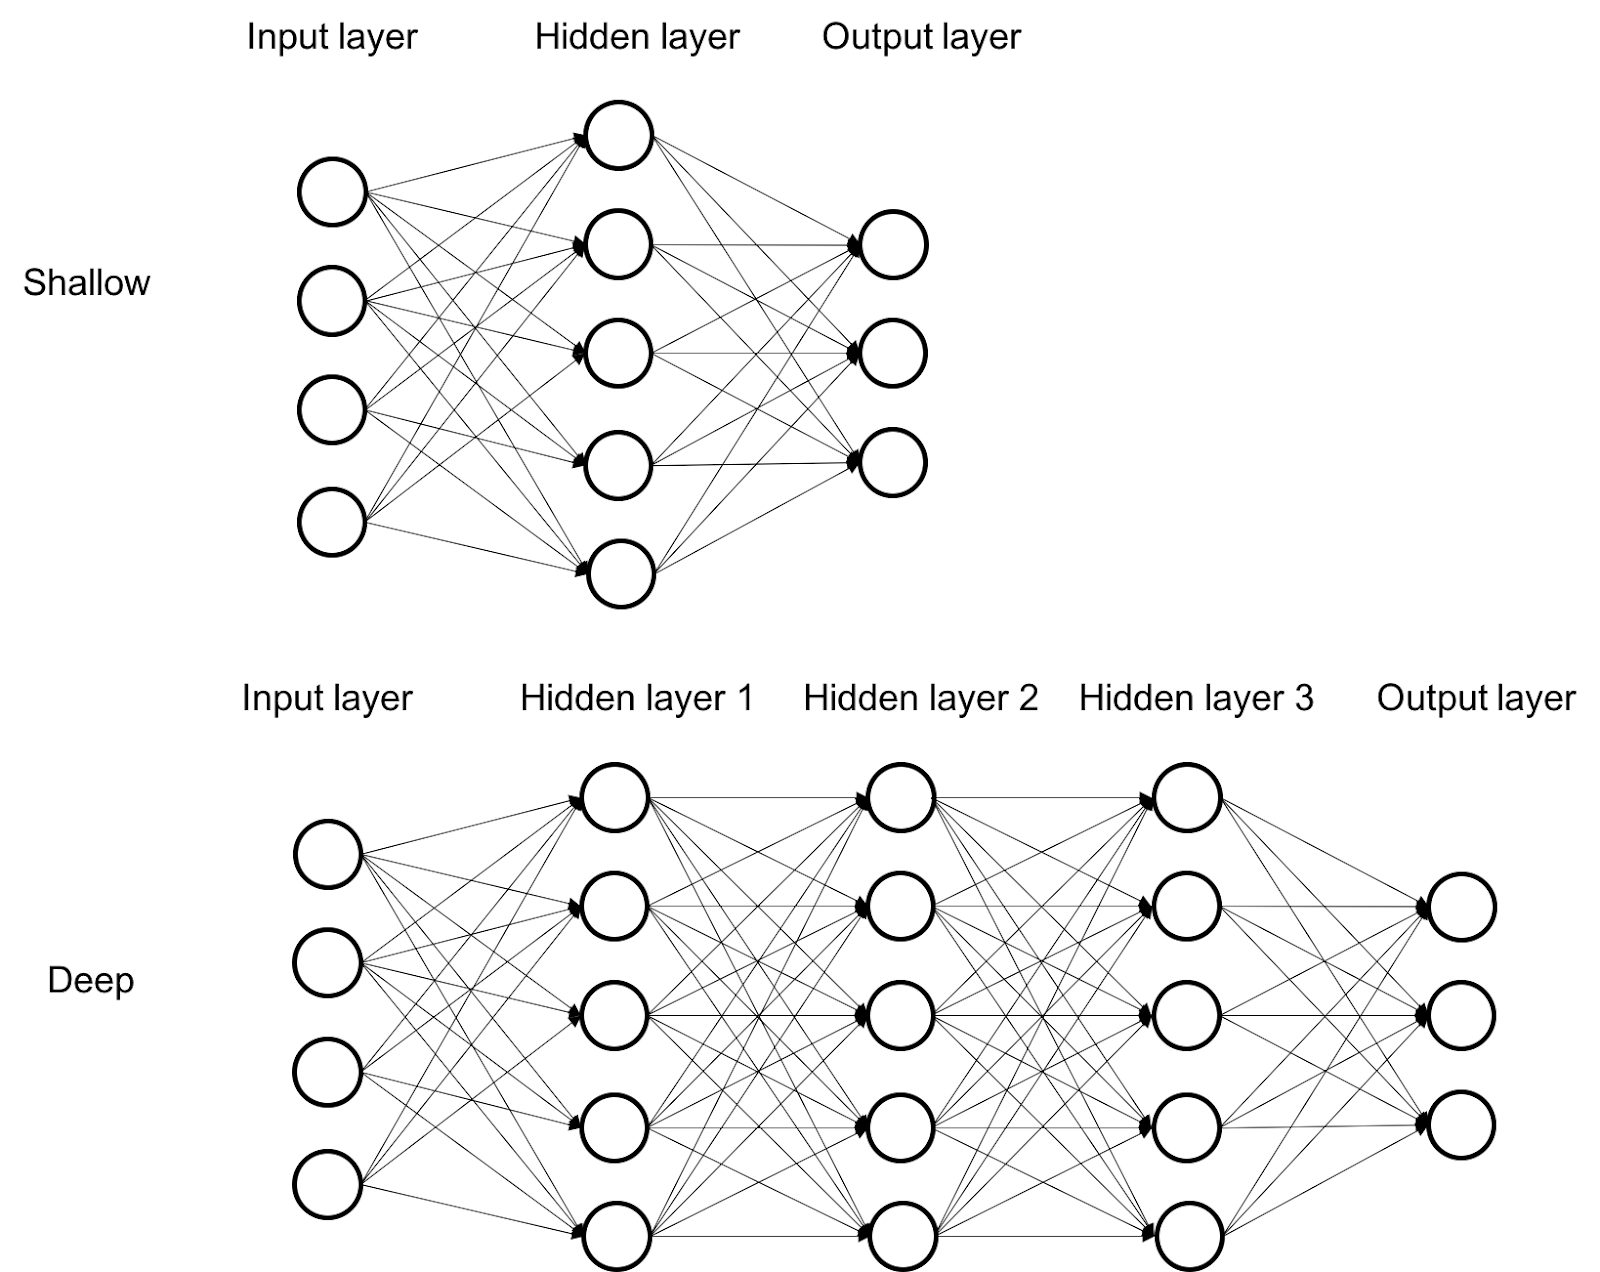
\includegraphics[width=0.8\linewidth]{Images/04_Images/shallow&deep_nn.png}
    \caption{Mạng nơ-ron nông và mạng nơ-ron sâu}
\end{figure}

Đối với mạng nơ-ron sâu, nhiều lớp ẩn được sử dụng để xây dựng một chuỗi các biểu diễn trung gian. Trong nhiều kiến trúc, các lớp ở những vị trí khác nhau có thể học các mức độ biểu diễn khác nhau: các lớp gần đầu vào thường mã hóa những đặc trưng có quan hệ trực tiếp hơn với dữ liệu ban đầu, trong khi các lớp sâu hơn có khả năng kết hợp các biểu diễn trước đó để hình thành những đặc trưng có mức độ trừu tượng cao hơn. Cấu trúc biểu diễn phân cấp này cho phép mạng mô hình hóa các quan hệ phức tạp thông qua nhiều phép biến đổi được hợp thành, và là một đặc điểm quan trọng của học sâu.

Tuy nhiên, việc gia tăng chiều sâu cũng làm tăng độ phức tạp của quá trình tính toán và tối ưu hóa. Trong lan truyền ngược của các mạng sâu, quá trình lan truyền gradient của hàm mất mát đối với các tham số của mạng qua nhiều lớp liên tiếp có thể dẫn đến hiện tượng suy giảm hoặc bùng nổ gradient, gây khó khăn cho quá trình huấn luyện. Những tiến bộ về kiến trúc mạng, hàm kích hoạt, thuật toán tối ưu, kỹ thuật khởi tạo tham số, chuẩn hóa và phần cứng tính toán song song đã góp phần khắc phục các hạn chế này, qua đó cho phép huấn luyện các mô hình học sâu với quy mô ngày càng lớn.
